% =====================================================================
%  ETSI GS QKD 018: SDN orchestration of multi-domain QKD networks
%  ---------------------------------------------------------------------
%  BUILD (XeLaTeX or LuaLaTeX, NOT pdfLaTeX):
%      latexmk -xelatex main.tex
%  or, by hand:
%      xelatex main.tex ; biber main ; xelatex main.tex ; xelatex main.tex
%  The math font is Cambria Math (unicode-math, \setmathfont), shipped
%  with Windows and Microsoft Office. If it is missing (e.g. on
%  Overleaf) Latin Modern Math is used automatically.
%  On Overleaf: Menu -> Compiler -> XeLaTeX.
%
%  Project layout:
%      main.tex           main document
%      preamble.tex       packages, fonts, environments
%      abstract/          abstract
%      chapters/          one file per section
%      figures/           TikZ figures
%      bibliography/      references.bib
% =====================================================================
\documentclass[11pt,a4paper]{article}
% =====================================================================
%  Preamble: packages, fonts, environments and styles
% =====================================================================

% ---------- Fonts and language (requires XeLaTeX or LuaLaTeX) ----------
\usepackage{fontspec}
\usepackage{amsmath,amssymb}
\usepackage{amsthm}
\usepackage{unicode-math}
\usepackage[english]{babel}
\usepackage{csquotes}

% Cambria Math for math environments; fallback if not installed
\IfFontExistsTF{Cambria Math}
  {\setmathfont{Cambria Math}}
  {\setmathfont{Latin Modern Math}}
% To typeset the body text in Cambria as well, uncomment:
% \IfFontExistsTF{Cambria}{\setmainfont{Cambria}}{}

% ---------- Layout ----------
\usepackage[a4paper,margin=2.5cm]{geometry}
\usepackage{microtype}
\usepackage{booktabs,tabularx,array,longtable}
\usepackage{enumitem}
\usepackage[font=small,labelfont=bf]{caption}
\usepackage{xcolor}
\usepackage{listings}
\usepackage{tikz}
\usetikzlibrary{arrows.meta,positioning,fit,calc,shapes.geometric,backgrounds}
\usepackage{authblk}

% ---------- Bibliography ----------
\usepackage[backend=biber,style=numeric-comp,sorting=none,maxbibnames=6]{biblatex}
\addbibresource{bibliography/references.bib}

\usepackage[hidelinks]{hyperref}
\usepackage{xurl}

% every section starts on a new page
\usepackage{etoolbox}
\pretocmd{\section}{\clearpage}{}{}

\setlist{itemsep=2pt,topsep=4pt}
\setlength{\parskip}{3pt}
\setlength{\emergencystretch}{2em}
\newcolumntype{L}{>{\raggedright\arraybackslash}X}
% allow line breaks after underscores in \texttt identifiers
\AtBeginDocument{\renewcommand{\_}{\textunderscore\allowbreak}}

% ---------- "definition" environment ----------
\theoremstyle{definition}
\newtheorem{definition}{Definition}[section]

% ---------- Listings (YANG, pyang trees, JSON, HTTP) ----------
\definecolor{codebg}{gray}{0.96}
\definecolor{codekw}{RGB}{0,70,140}
\definecolor{codecm}{RGB}{110,110,110}
\definecolor{codestr}{RGB}{150,40,40}
\lstdefinelanguage{yang}{
  morekeywords={module,namespace,prefix,import,organization,contact,
    description,revision,reference,yang-version,identity,base,typedef,type,
    identityref,grouping,uses,container,list,key,leaf,leaf-list,config,
    augment,rpc,input,output,notification,leafref,path,default,units,
    must,when,enum,enumeration,mandatory},
  sensitive=true,
  morecomment=[l]{//},
  morecomment=[s]{/*}{*/},
  morestring=[b]"
}
\lstdefinestyle{code}{
  basicstyle=\ttfamily\footnotesize,
  keywordstyle=\color{codekw}\bfseries,
  commentstyle=\color{codecm}\itshape,
  stringstyle=\color{codestr},
  backgroundcolor=\color{codebg},
  frame=single, framerule=0pt,
  columns=fullflexible, keepspaces=true,
  xleftmargin=4pt, xrightmargin=4pt,
  breaklines=true, upquote=true,
  aboveskip=6pt, belowskip=6pt
}
\lstset{style=code}

% ---------- Shared TikZ styles ----------
\tikzset{
  >=Stealth,
  box/.style={draw,rounded corners,minimum height=8mm,align=center,
              font=\small},
  lbl/.style={font=\scriptsize,midway,fill=white,inner sep=1pt},
  actor/.style={draw,rounded corners,fill=gray!8,minimum width=2.4cm,
                minimum height=7mm,align=center,font=\small},
  msg/.style={->,thick},
  ret/.style={->,dashed}
}


\title{\textbf{SDN Orchestration of Multi-Domain QKD Networks:\\
       the ETSI GS QKD 018 Interface}}
\author{Diego Carro}
\author{Bucci Felice Elia}
\affil{Cybersecurity course, Politecnico di Torino\\Quantum Engineering}
\date{November 2026}

\begin{document}
\maketitle

% =====================================================================
%  Abstract
% =====================================================================
\begin{abstract}
\noindent
Quantum key distribution (QKD) lets two parties agree on a secret key whose
security rests on the laws of physics rather than on computational
hardness. Moving it from the laboratory into an operator's network,
however, means managing it like any other network resource: discovering its
topology, monitoring its state, allocating its capacity to services and
coordinating it with classical networks. The ETSI ISG QKD addressed this
problem step by step. GS~QKD~002 identifies the use cases and integration
requirements; GS~QKD~015 defines the model through which an SDN controller
sees and configures the QKD nodes of a domain; GS~QKD~018 defines the
interface between an \emph{SDN orchestrator} and the controller of a QKD
domain, enabling end-to-end provisioning across several domains and
between a QKD network and an optical transport network. This work follows
that chain in a reasoned way: it describes the components of an SD-QKD
network and the structure of a YANG model, analyses GS~QKD~018 in detail
(use cases, information model, topology, inventory and connectivity
modules, multi-domain workflow, security), shows its analogy with the IETF
ACTN framework (RFC~8453) and compares it with three real experiences: SK
Telecom's multi-vendor KOREN testbed, an ONOS-based hierarchical prototype
developed at Politecnico di Milano, and the MadQCI network in Madrid. It
closes with the current limits of the standard and open research
directions.

\medskip
\noindent\textbf{Keywords:} QKD, SDN, orchestration, ETSI GS QKD 015,
ETSI GS QKD 018, YANG, RESTCONF, multi-domain, key management.
\end{abstract}


\tableofcontents
\bigskip

% =====================================================================
\section{State of the art}
\label{sec:sota}
% =====================================================================

\paragraph{QKD fundamentals.}
The QKD literature is by now well established. The review by Pirandola
et al.~\cite{pirandola2020} covers discrete-variable protocols (BB84 and
its \emph{decoy-state} variants), continuous-variable protocols and
security proofs. Two constraints that drive all network engineering emerge
from it: the key rate decays exponentially with distance, and a single
link over commercial fibre does not exceed a few hundred kilometres.

\paragraph{From link to network.}
Mehic et al.~\cite{mehic2020} and Cao et al.~\cite{cao2022} describe the
transition from point-to-point links to QKD \emph{networks}: layered
architecture, \emph{trusted relay}, key management and routing. The GÉANT
white paper~\cite{geant2024} gives a readable summary of the same picture
and of the ETSI and ITU-T standards. Routing, which becomes central once a
network is orchestrated, is discussed in~\cite{routing2024}.

\paragraph{Standardisation.}
Two bodies have produced complementary specifications. ETSI ISG QKD started
in 2010 with the use cases~\cite{qkd002} and then defined the interfaces
towards applications~\cite{qkd004,qkd014}, towards the SDN
controller~\cite{qkd015}, towards the orchestrator~\cite{qkd018} and
between key management systems~\cite{qkd020}. ITU-T, with the Y.3800
series, defined the reference architecture of QKD networks
(QKDN)~\cite{ituy3800}, their control and management~\cite{ituy3804} and
SDN-based control~\cite{ituy3805}.

\paragraph{SDN applied to QKD.}
The \emph{Software-Defined Networking} paradigm~\cite{kreutz2015} separates
the control plane from the data plane and centralises decisions in a
programmable controller. The UPM/Telefónica group was the first to
integrate QKD resources into an SDN-controlled optical network, both
experimentally~\cite{aguado2016} and in a systematic
tutorial~\cite{aguado2020}; GS~QKD~015 grew out of this line of work.

\paragraph{Orchestration and multi-domain.}
The orchestrator–controller interface is specified by
GS~QKD~018~\cite{qkd018} and its YANG modules~\cite{qkd018yang}. The first
documented real deployment is that of Sim et al.~\cite{sim2023} (SK
Telecom), who orchestrate two domains from different vendors on the KOREN
testbed. Vicario's thesis~\cite{vicario2025} builds a complete hierarchical
prototype with ONOS and RESTCONF. The MadQCI network~\cite{madqci2024} uses
GS~QKD~015 extensively but describes GS~QKD~018 orchestration as work still
in progress. More recent works propose SDN applications for dynamic link
reconfiguration~\cite{mendez2026}, path-selection criteria and inter-domain
routing that preserves topology confidentiality~\cite{laschet2026}, and
hybrid key-delivery models between regional networks~\cite{interconnect2026}.

\paragraph{Contribution.}
With respect to these sources, this work offers a unified and reasoned
reading of the GS~QKD~002 $\to$ 015 $\to$ 018 chain: it shows how the
requirements of the use cases translate into the components of an SD-QKD
network, explains the structure of the YANG models that describe them and
analyses how GS~QKD~018 abstracts them for multi-domain orchestration.

% =====================================================================
\section{Introduction}
\label{sec:intro}
% =====================================================================

This section builds the vocabulary needed to read the ETSI specifications.
It starts from QKD as a cryptographic primitive, moves on to QKD networks
with their trusted nodes and layered architecture, recalls the essential
concepts of SDN and finally reaches the two documents that precede
GS~QKD~018: GS~QKD~002 (§\ref{sec:qkd002}) and GS~QKD~015
(§\ref{sec:qkd015}).

\paragraph{Quantum key distribution.}

\begin{definition}[QKD]
\emph{Quantum Key Distribution} is a procedure that, through the transport
of quantum states, allows two remote parties to agree on shared secret bit
strings, with security based on entanglement or on the impossibility of
perfectly cloning or measuring unknown quantum states~\cite{qkd018}.
\end{definition}

BB84 makes the idea clear. Alice encodes random bits on single photons in
one of two randomly chosen bases; Bob measures in a basis that is also
random; over an \emph{authenticated} classical channel the two compare bases
and keep only the bits measured in the right one (\emph{sifting}). An
eavesdropper who measures the photons unavoidably introduces errors,
quantified by the \emph{Quantum Bit Error Rate}
\begin{equation}
  \mathrm{QBER} = \frac{N_{\text{errors}}}{N_{\text{sifted}}} .
\end{equation}
If the QBER stays below a threshold (about $11\%$ for BB84 against
collective attacks), error correction and \emph{privacy amplification}
distil a secret key; otherwise the block is discarded. The quantity the
network cares about is the \emph{secret key rate} (SKR), the number of
secure key bits produced per second. Since fibre transmittance decays as
$\eta = 10^{-\alpha L/10}$, with $\alpha \approx 0.2$~dB/km, the SKR also
drops quickly with the link length $L$.

Two observations, which we will meet again in the GS~QKD~002 use cases,
are fundamental. QKD \emph{distributes} keys but neither encrypts nor
authenticates: it must always be combined with a cipher (one-time pad or
AES) and an authentication mechanism. Moreover, the classical channel must
be authenticated from the very first exchange, which requires a small
pre-shared secret: strictly speaking QKD is a \emph{key growing} mechanism.

\paragraph{From link to network: the trusted node.}
A QKD link spans at most a few hundred kilometres and practical quantum
repeaters do not exist yet. Real networks therefore chain links through
trusted nodes.

\begin{definition}[Trusted node and key relay]
A \emph{trusted node} is a node, located inside a physically protected
perimeter, that shares QKD keys with both its neighbours. To carry a key
$K$ from $A$ to $C$ through $B$, node $A$ sends $c = K \oplus K_{AB}$; $B$
computes $K = c \oplus K_{AB}$ and forwards $c' = K \oplus K_{BC}$. Each hop
is \emph{one-time pad} encrypted, but $K$ appears in the clear inside every
intermediate node, which must therefore be trusted.
\end{definition}

Note that relaying consumes key: to carry $|K|$ bits along a path $p$, every
link $\ell\in p$ spends $|K|$ bits of its own local key. This simple fact
turns key into a \emph{network resource} that must be planned, and it is why
the later specifications talk about available rates, consumption and paths.

\paragraph{The ITU-T layered architecture.}
Recommendation ITU-T Y.3800~\cite{ituy3800} organises a QKD network (QKDN)
into stacked layers (Fig.~\ref{fig:itu}): the \emph{quantum layer} with
the QKD modules; the \emph{key management layer} with the key managers that
store and relay keys; the \emph{control layer}, which takes operational
decisions (routing, relay, link configuration); the \emph{management
layer}, which supervises everything; and the \emph{service layer}, where
applications consume keys. Two kinds of link are distinguished in this
scheme.

\begin{definition}[QKD link and KM link]
A \emph{QKD link} connects two QKD modules and consists of a quantum
channel and a classical channel: it is where key is \emph{generated}. A
\emph{KM link} connects two \emph{key managers}: it is the classical
channel, protected with QKD keys, along which key is \emph{relayed}.
\end{definition}

Likewise, two roles that are often confused are kept apart. The \emph{QKDN
controller} acts on the network in real time: it decides relay paths,
enables or disables links and reacts to failures. The \emph{QKDN manager}
has a supervisory role: it collects FCAPS information (\emph{Fault,
Configuration, Accounting, Performance, Security}) and enforces policies.
The ETSI specifications discussed below sit in the control plane:
GS~QKD~015 between controller and nodes, GS~QKD~018 between controller and
orchestrator.

% Figure: layered architecture of a QKDN (ITU-T Y.3800)
\begin{figure}[t]
\centering
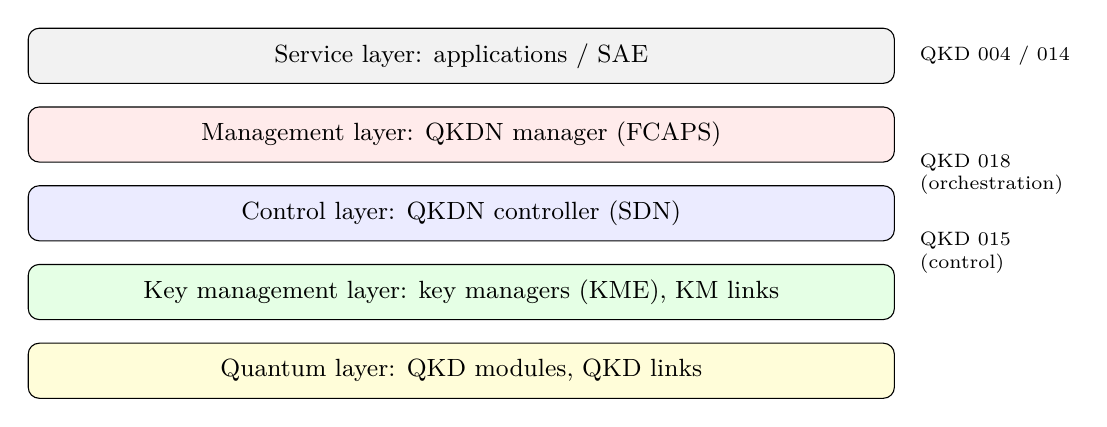
\begin{tikzpicture}[
  layer/.style={draw,rounded corners,minimum width=11cm,minimum height=7mm,
                align=center,font=\small},
  side/.style={font=\scriptsize,align=left,anchor=west}]
  \node[layer,fill=gray!10]   (srv) at (0,0)    {Service layer: applications / SAE};
  \node[layer,fill=red!8]     (mgm) at (0,-1.0) {Management layer: QKDN manager (FCAPS)};
  \node[layer,fill=blue!8]    (ctl) at (0,-2.0) {Control layer: QKDN controller (SDN)};
  \node[layer,fill=green!10]  (km)  at (0,-3.0) {Key management layer: key managers (KME), KM links};
  \node[layer,fill=yellow!15] (q)   at (0,-4.0) {Quantum layer: QKD modules, QKD links};
  \node[side] at (5.7,0)    {QKD 004 / 014};
  \node[side] at (5.7,-1.5) {QKD 018\\(orchestration)};
  \node[side] at (5.7,-2.5) {QKD 015\\(control)};
\end{tikzpicture}
\caption{Layered architecture of a QKD network according to ITU-T
Y.3800~\cite{ituy3800}; on the right, the indicative position of the ETSI
specifications discussed in the text.}
\label{fig:itu}
\end{figure}


Applications do not see the quantum part. A \emph{Secure Application
Entity} (SAE) requests keys from the \emph{Key Management Entity} (KME) of
its node through the GS~QKD~004~\cite{qkd004} or GS~QKD~014~\cite{qkd014}
APIs; two SAEs that want to communicate obtain the same key from their
respective KMEs, identified by a \emph{key ID}.

\paragraph{Software-Defined Networking.}
In a traditional network each device decides on its own how to forward
traffic. SDN~\cite{kreutz2015} instead separates three planes: the
\emph{data plane}, made of devices that execute; the \emph{control plane},
centralised in a controller with a global view of the network; and the
\emph{management and application plane}, which expresses goals. The
controller talks to the devices through a \emph{southbound} interface (SBI)
and offers its services upwards through a \emph{northbound} interface
(NBI). When there is more than one domain, an \emph{orchestrator} is added
above the controllers to coordinate end-to-end services without knowing
the details of each domain.

A QKD network has every feature that makes SDN useful: scarce and variable
resources (the key), tight physical constraints (attenuation, coexistence
with classical channels), multi-vendor equipment and demand that changes
over time. The two specifications that follow describe why and how ETSI
applied this paradigm to QKD.

% =====================================================================
\subsection{ETSI GS QKD 002: the use cases}
\label{sec:qkd002}
% =====================================================================

GS~QKD~002 V1.1.1 (June 2010)~\cite{qkd002} is the first document published
by the ISG QKD. Its goal is not strictly technical: before standardising
\emph{how} to implement QKD, the group wanted to clarify \emph{where} it is
needed, \emph{who} uses it and \emph{which requirements} it must meet to
enter existing infrastructures. The document reasons in three steps: it
places QKD among cryptographic primitives, identifies the layers of the
network stack where it can be inserted and describes six use cases with
their requirements. Following this reasoning is useful because it shows
where the needs come from that, twelve years later, led to GS~QKD~015
and~018.

\subsubsection{QKD as a cryptographic primitive}

The document starts from a typical QKD system: two units, usually 19"
rack-mounted, connected by a quantum channel over fibre or free space up to
about $100$~km long, which output the same random bit sequence at both
ends. Clause 4 immediately makes clear that this solves \emph{a single}
cryptographic problem.

A secure system needs three primitives: \emph{encryption}, \emph{key
distribution} and \emph{message authentication}. QKD covers only the
second; encryption requires a one-time pad or symmetric ciphers such as
AES, and authentication requires MACs (for instance based on Wegman–Carter
universal hashing) or digital signatures. It follows that QKD is a
\emph{complement} to classical cryptography, not a replacement, and that
its overall security also depends on the other components of the system.
The document also stresses that the public channel of QKD must be
authenticated with a pre-distributed secret.

\subsubsection{Where QKD fits in the network stack}

Clause 6 describes at which layer of the stack a QKD key can be consumed.
The choice of layer determines what must be modified and how transparent
the integration is.

\begin{description}[style=nextline,leftmargin=1.2em]
  \item[Data link layer (L2)] The QKD key feeds the PPP key exchange, the
        IEEE~802.1AE (MACsec) keys or a \emph{QKD link encryptor}, i.e.\ a
        line encryptor that directly consumes the keys produced by the link
        and creates an encrypted tunnel between two sites. It is the most
        transparent option for applications.
  \item[Network layer (L3)] A modified IKE uses the QKD key as the shared
        secret for IPsec.
  \item[Transport layer (L4)] The QKD key replaces the TLS/SSL session keys
        or is used instead of HMACs for authentication.
  \item[Application layer] Applications use the key to authenticate users
        or to encrypt the content exchanged between their instances.
\end{description}

The conceptual point is that, whatever the layer, there is one component
that \emph{consumes} keys and one that \emph{supplies} them: this is the
separation that later becomes SAE and KME, with a standard interface
(GS~QKD~004 and~014) between them.

\subsubsection{The six use cases}

Clause 7 describes six use cases with a fixed structure: goal,
description, actors, benefits, operational and quality-of-service
considerations. We summarise them along a logical thread: from a single
link to a network, and from a private network to an operator's network.

\paragraph{UC1 – Offsite backup / business continuity.}
An enterprise replicates data from a primary site to a backup site (daily
backups, snapshots, SAN mirroring, database replication). A single
point-to-point QKD link feeds a line encryptor over Ethernet or Fibre
Channel; the fibre may be dedicated (\emph{dark fibre}) or shared via WDM
or TDM. The requirements that emerge are: key renewal as frequent as the
generation rate allows, handling of recalibration phases during continuous
transfers, an initial secret at installation, and high encryption speed.
The document notes that overall security is not unconditional, since it
also depends on the encryptor.

\paragraph{UC2 – Enterprise metropolitan area network.}
Several branches of an enterprise or a public body are connected to data
centres, through which branch-to-branch traffic also flows. Each link is
protected by a QKD link encryptor that encrypts and authenticates at
layer~2, transparently for applications. Two new needs appear: different
links carry different traffic volumes and timings, hence \emph{different
QoS requirements}, and transfers may be scheduled, periodic or triggered by
thresholds. The \emph{QKD Secured Key Server} variant has a central server
that distributes keys and certificates to clients across the metropolitan
area over channels encrypted with one-time pad and authenticated with
Wegman–Carter: an early example of a key service offered by a network.

\paragraph{UC3 – Critical infrastructure control and data acquisition.}
This case protects the SCADA traffic of a critical infrastructure, with a
railway network as the example: here the \emph{authenticity} of commands
(switches, signals) matters more than their confidentiality. The nodes of
the private WAN sit in stations with a controlled perimeter, while the
fibre lies outside it. The document proposes two architectures: single QKD
links between nodes, with key buffering and forwarding handled in the
nodes, or a \emph{QKD network with integrated key management} and a
dedicated interface towards applications. It asks for the highest
availability, with precautions for recalibration, failures and denial of
service, and for the ability to initialise new redundant links with secrets
obtained along an alternative path. It is the first case in which key
relay, centralised management and path redundancy appear together.

\paragraph{UC4 – Backbone protection.}
A fibre in an operator's metropolitan backbone, typically a WDM ring with
OADMs or ROADMs, carries a quantum channel alongside the data channels. The
keys protect control and management traffic or are offered to customers.
There are two actors: the infrastructure provider and the service provider
that uses it; backbone nodes are trusted. The requirements are the closest
to those of an operator: the QKD system must not reduce the throughput of
the WDM system by more than $10\%$, must be compatible with common fibres,
splices and connectors, its management must \emph{integrate into the
management of the WDM system}, and installation and maintenance must be
possible for staff without quantum physics expertise.

\paragraph{UC5 – High-security access network.}
In a passive optical network (PON) for Fiber-to-the-Home, downstream traffic
is broadcast to all ONUs, so it must be encrypted to prevent one user from
reading another's data. One OLT serves $32$ to $128$ ONUs and the quantum
channel follows the same path as the classical one. The configuration is
highly asymmetric: a single, more expensive detector at the OLT serves many
sources at the ONUs. Short distances allow high rates, which are needed
because the generation capacity is shared among all users. The \emph{QKD
Authenticated Sensor Network} variant applies the same scheme to a central
station with many sensors and actuators.

\paragraph{UC6 – Long-haul service.}
Two distant ground stations $A$ and $B$, for example on opposite shores of
an ocean, want to share a key without trusting intermediate ground nodes. A
moving node $C$ (satellite, aircraft or high-altitude platform) establishes
a secret $a$ with $A$ and then a secret $b$ with $B$, and sends $a\oplus b$
to $B$ over a classical channel; $B$ recovers $a$. It is a key relay in
which the trusted node is $C$. Low-orbit satellites fly at about
$300$–$800$~km and pass over the stations about once a day; geostationary
orbit is not practical. Weather and atmosphere can reduce or cancel the
rate, so redundant channels are needed.

Table~\ref{tab:qkd002} summarises the six cases.

\begin{table}[h]
\centering\small
\caption{The GS~QKD~002 use cases and the elements that anticipate later
specifications.}
\label{tab:qkd002}
\begin{tabularx}{\textwidth}{@{}l L L@{}}
\toprule
\textbf{Case} & \textbf{Configuration} & \textbf{Need it anticipates} \\
\midrule
UC1 Backup & point-to-point link + line encryptor & key–encryptor interface \\
UC2 Enterprise metro & several links, key server & per-application QoS \\
UC3 Critical infrastructure & network with key relay and integrated management & KMS, redundancy, centralised control \\
UC4 Backbone & quantum channel in WDM & coexistence with the optical network, integrated management \\
UC5 PON access & point-to-multipoint & sharing of key capacity \\
UC6 Long-haul & relay through a moving node & trusted node, redundancy \\
\bottomrule
\end{tabularx}
\end{table}

\subsubsection{What it leaves behind}

GS~QKD~002 is a first-edition document: the clause on general requirements
and the functional characteristics of the individual cases are marked as
not yet available. Its value lies in having set the questions. Read in
sequence, the use cases show that useful QKD is not a single link but a
\emph{network}, which requires: a key management system that stores and
relays keys (UC3, UC6); a way to express different service requirements for
different applications (UC2); and coexistence with the operator's optical
network, with management integrated into the existing one and usable by
non-specialist staff (UC4). The first two needs are answered by GS~QKD~015,
the third, in the form of coordination between the QKD network and the
transport network, by GS~QKD~018.

% =====================================================================
\subsection{ETSI GS QKD 015: the SDN controller and the SD-QKD network}
\label{sec:qkd015}
% =====================================================================

GS~QKD~015 (V1.1.1 in 2021, V2.1.1 in April 2022)~\cite{qkd015} defines
the control interface between an SDN controller and the nodes of a QKD
network, i.e.\ the \emph{southbound interface} of the QKD control plane.
The second edition, considered here, was aligned with GS~QKD~018: the
GS~QKD~018 YANG modules import those of GS~QKD~015 directly. A good
understanding of 015 is therefore a prerequisite for understanding 018.

The section proceeds in four steps: why software control is needed; what
the components of an SD-QKD network are, one by one; what a YANG model
looks like in general; and how 015 uses YANG to describe the node, with the
resulting workflows and security considerations.

% ---------------------------------------------------------------------
\subsubsection{Why software-defined control}

The specification starts from an observation: integrating QKD into a
telecommunications network is today a manual operation. Each new QKD
system is installed by hand, usually over a dedicated dark fibre between
two sites, forming a fixed link. This approach has three limits. It does
not scale, because every change requires human intervention. It wastes
resources, because the key capacity of a link cannot be moved to where it
is needed. And it does not talk to the optical network, which is
increasingly disaggregated and software-controlled.

The proposed architecture lets a controller orchestrate QKD resources
centrally: optimise the key allocation per link according to demand,
automatically create direct or multi-hop links, and coordinate quantum and
classical channels even when they share the same fibre. In particular, the
abstraction defined by the specification aims to:
\begin{itemize}
  \item manage QKD resources centrally according to demands, capabilities
        and network state;
  \item aggregate the QKD systems of the same perimeter under a single key
        management, to better detect demands;
  \item hide the complexity of the low-level parameters of each technology,
        delegating them to the node;
  \item optimise the distribution of links according to application QoS and
        generation statistics;
  \item coordinate quantum and classical channels, whether or not they
        share the same physical medium.
\end{itemize}
These are, in technical form, the needs that emerged from use cases UC2,
UC3 and UC4 of GS~QKD~002.

% ---------------------------------------------------------------------
\subsubsection{The components of an SD-QKD network}

It is convenient to build the network bottom-up, adding one abstraction at
a time. Fig.~\ref{fig:sdqkd} shows the result.

\paragraph{1. QKD module, system and link.}
The basic physical unit is the \emph{QKD module}: the set of hardware and
software that runs part of a QKD protocol. Two connected modules form a
\emph{QKD system}, and the connection between them (quantum channel plus
classical channel) is the \emph{QKD link}. So far we are in the quantum
layer of Fig.~\ref{fig:itu}: modules are vendor- and technology-specific
(discrete or continuous variables, encoding, wavelength) and do not
interoperate.

\paragraph{2. QKD interface.}
The controller does not need to know how a module works internally, only
what it offers to the network. GS~QKD~015 therefore introduces an
abstraction.

\begin{definition}[QKD interface]
A \emph{QKD interface} (\texttt{qkdi}) is the abstract representation of a
QKD module within a node: it exposes only the attributes relevant to the
network, such as technology, model, wavelength range, maximum supported
attenuation and attachment point to an optical switch.
\end{definition}

The analogy is the ports of a switch: a node with three QKD modules appears
to the controller as a device with three interfaces. Since modules from
different vendors do not interoperate, the model requires the technology
and model of each interface to be declared: the controller will pair only
compatible interfaces.

\paragraph{3. SD-QKD node.}
Interfaces located in the same secure site are grouped together.

\begin{definition}[SD-QKD node]
An \emph{SD-QKD node} is the aggregation of one or more QKD modules located
in a secure site and managed by a single \emph{SDN agent}, which exposes
them to the controller as a single network element with several interfaces.
\end{definition}

The specification sets a series of requirements that give the node its
shape. An SD-QKD node \emph{shall}: comprise at least one QKD module,
exposed as an interface; be located in a secure site (a site may host
several nodes); contain a \emph{key management system} that aggregates the
material produced by all key associations; offer applications a
\emph{single access point} to keys through an API; and connect to at least
one SDN controller via standard protocols for discovery, control and
telemetry. It \emph{should} also expose to the controller information on
applications, interfaces, links and classical-channel requirements (for
example acceptable attenuation).

Inside the node four logical components can thus be identified:
\begin{itemize}
  \item the \textbf{QKD modules}, which generate key with remote nodes;
  \item the \textbf{key manager} (KMS), which receives keys from the
        modules, stores them in one or more logical \emph{key stores},
        relays them when needed and registers applications with their QoS;
  \item the \textbf{application interface}, i.e.\ the key delivery API
        (GS~QKD~004 or~014), reachable at a known IP address and port;
  \item the \textbf{SDN agent}, which translates the state of all of the
        above into a YANG model, exposes it to the controller, receives
        configurations and sends notifications.
\end{itemize}

% Figure: SD-QKD network and internal structure of a node (adapted from GS QKD 015, Fig. 1)
\begin{figure}[t]
\centering
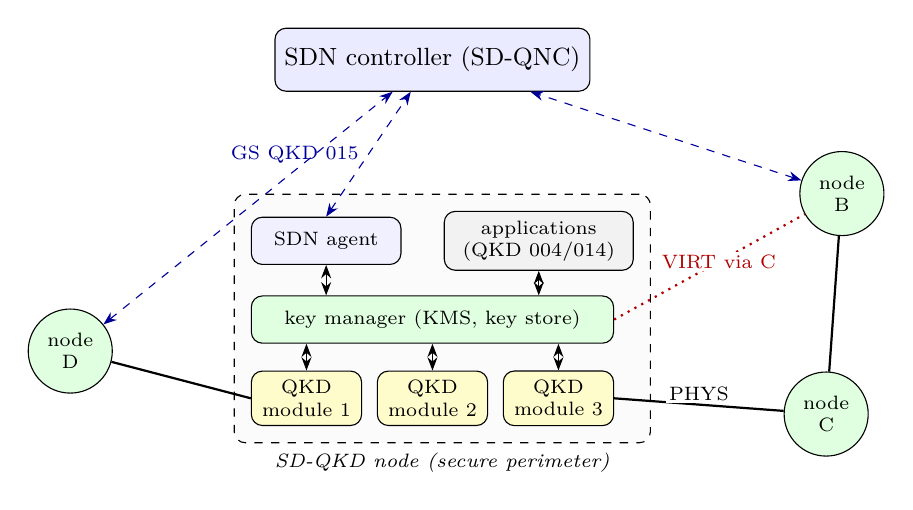
\begin{tikzpicture}[
  comp/.style={draw,rounded corners,align=center,font=\scriptsize,
               minimum height=6mm},
  small/.style={draw,circle,fill=green!12,minimum size=9mm,font=\scriptsize,
                align=center}]
  % controller
  \node[box,fill=blue!8,minimum width=4cm] (ctl) at (-0.6,4.3) {SDN controller (SD-QNC)};
  % detailed node
  \node[comp,fill=yellow!20,minimum width=1.4cm] (m1) at (-2.2,0) {QKD\\module 1};
  \node[comp,fill=yellow!20,minimum width=1.4cm] (m2) at (-0.6,0) {QKD\\module 2};
  \node[comp,fill=yellow!20,minimum width=1.4cm] (m3) at (1.0,0) {QKD\\module 3};
  \node[comp,fill=green!12,minimum width=4.6cm] (kms) at (-0.6,1.0) {key manager (KMS, key store)};
  \node[comp,fill=blue!6,minimum width=1.9cm] (agent) at (-1.95,2.0) {SDN agent};
  \node[comp,fill=gray!10,minimum width=2.4cm] (app) at (0.75,2.0) {applications\\(QKD 004/014)};
  \begin{scope}[on background layer]
    \node[draw,dashed,rounded corners,fill=gray!3,inner sep=6pt,
          fit=(m1)(m3)(kms)(agent)(app),
          label={[font=\scriptsize\itshape]below:SD-QKD node (secure perimeter)}] (node) {};
  \end{scope}
  % remote nodes
  \node[small] (r1) at (4.6,2.6) {node\\B};
  \node[small] (r2) at (4.4,-0.2) {node\\C};
  \node[small] (r3) at (-5.2,0.6) {node\\D};
  % links
  \draw[thick] (m3.east) -- node[lbl,above]{PHYS} (r2);
  \draw[thick] (m1.west) -- (r3);
  \draw[thick] (r1) -- (r2);
  \draw[thick,dotted,red!70!black] (kms.east) -- node[pos=0.55,font=\scriptsize,fill=white,inner sep=1pt]{VIRT via C} (r1);
  \draw[<->] (m1) -- (m1|-kms.south);
  \draw[<->] (m2) -- (m2|-kms.south);
  \draw[<->] (m3) -- (m3|-kms.south);
  \draw[<->] (agent.south) -- (agent.south|-kms.north);
  \draw[<->] (app.south) -- (app.south|-kms.north);
  \draw[<->,dashed,blue!60!black] (agent.north) -- node[pos=0.5,left,font=\scriptsize]{GS QKD 015} (ctl);
  \draw[<->,dashed,blue!60!black] (r1) -- (ctl);
  \draw[<->,dashed,blue!60!black] (r3) -- (ctl);
\end{tikzpicture}
\caption{An SD-QKD network: nodes are connected by physical (solid) and
virtual (dotted) links, and each is controlled by the controller through its
SDN agent (dashed). The node in the foreground shows the internal
components: the QKD modules, exposed as interfaces, the key manager, the
application interface and the agent. Adapted from~\cite[Fig.~1]{qkd015}.}
\label{fig:sdqkd}
\end{figure}


\paragraph{4. Key association link.}
Between two nodes the interesting quantity is not the quantum channel
itself but the fact that the two nodes share key. GS~QKD~015 models exactly
this.

\begin{definition}[Key association link]
A \emph{key association link} (\texttt{qkd\_link}) is a logical key
association between two remote SD-QKD nodes. It is of type \texttt{PHYS}
(direct) if a quantum channel connects the two nodes, of type \texttt{VIRT}
(virtual) if the key is obtained by key relay through intermediate trusted
nodes.
\end{definition}

A physical link corresponds to a QKD link in ITU-T terminology; a virtual
link corresponds to a chain of KM links over several QKD links. Two details
make the model consistent. First, a virtual link \emph{consumes} key from
the physical links it rests on, and is therefore registered as an
\emph{internal application} with a reserved bandwidth
(\texttt{virt\_bandwidth}). Second, every intermediate node of a virtual
link knows the previous and the next node (\texttt{virt\_prev\_hop},
\texttt{virt\_next\_hop}), so the relay path is configured hop by hop by
the controller. For a node to act as a relay it must declare the
\texttt{key\_relay\_mode\_enable} capability.

\paragraph{5. Applications.}
From the node's point of view, an application is any entity that requests
keys from the key manager.

\begin{definition}[QKD application]
A \emph{QKD application} (\texttt{qkd\_app}) is a running instance that
consumes keys from an SD-QKD node. It is \emph{external}
(\texttt{CLIENT}) if it is a user, an HSM, an encryptor, a virtual network
function or a security protocol; it is \emph{internal}
(\texttt{INTERNAL}) if it uses keys for the operation of the network
itself, such as authentication or relay for a virtual link.
\end{definition}

Each application declares a quality of service: maximum and minimum key
bandwidth (\texttt{max\_bandwidth}, \texttt{min\_bandwidth}, in bit/s),
maximum delivery \texttt{jitter} in ms, lifetime \texttt{ttl} of an unused
key in the key store, and whether paths or keys may be shared among several
clients. This is the technical answer to the differentiated-QoS need of
UC2.

\paragraph{6. SDN controller.}
At the top sits the controller (in 015 also \emph{SD-QNC},
\emph{Software-Defined QKD Network Controller}), which has the global view
of the domain and plays three roles. It acts as the \emph{central registry}
of applications, so that an application only needs to know its own key
manager and not the network topology. It plans and creates \emph{links},
physical or virtual, according to demand and statistics. And it
coordinates its domain with the optical network controller
(\emph{SD-ONC}) when a new optical path is needed for a quantum channel.

\paragraph{What does not reach the controller.}
The information that crosses the control plane is deliberately minimal:
identifiers, states, rates, physical parameters. Key material \emph{never
leaves the node perimeter}. For this reason, the specification observes,
introducing SDN into a trusted-node network adds no new risks beyond those
already known, such as denial of service.

% ---------------------------------------------------------------------
\subsubsection{Anatomy of a YANG model}
\label{sec:yang-anatomia}

Both 015 and 018 are written in YANG~\cite{rfc7950}, a language born in the
IETF to describe the configuration and state data of network devices and
the operations that can be invoked on them. A YANG model is not executable
code: it is a \emph{schema}, like an XSD for XML or a JSON schema, which
states which data exist, of which type, how they are nested and who may
modify them. The NETCONF and RESTCONF protocols then work on top of that
schema. We go through the main constructs using examples taken from the
015 files~\cite{qkd015yang}.

\paragraph{The module and its header.}
The basic unit is the \emph{module}. Its header declares the language
version, a globally unique \texttt{namespace}, a short \texttt{prefix} used
by other modules to refer to it, the imported modules and the revisions.
\begin{lstlisting}[language=yang]
module etsi-qkd-sdn-node {
  yang-version "1";
  namespace "urn:etsi:qkd:yang:etsi-qkd-node";
  prefix "etsi-qkdn";
  import ietf-yang-types   { prefix "yang"; }
  import ietf-inet-types   { prefix "inet"; }
  import etsi-qkd-node-types { prefix "etsi-qkdn-types"; }
  organization "ETSI ISG QKD";
  revision "2022-01-30" { reference "ETSI GS QKD 015 V2.1.1"; }
  ...
}
\end{lstlisting}
GS~QKD~015 is split into two modules. The first one,
\texttt{etsi-qkd-node-types}, contains only types; the second one,
\texttt{etsi-qkd-sdn-node}, contains the actual model. This is
a common choice: separating the types lets other modules, such as those of
018, reuse them without importing everything else.

\paragraph{Types: built-in, typedef and identity.}
YANG offers built-in types (\texttt{boolean}, \texttt{string},
\texttt{uint32}, \texttt{decimal64}, \texttt{enumeration}\dots) and common
types defined by the IETF, such as \texttt{yang:uuid} or
\texttt{yang:date-and-time}. \texttt{typedef} defines derived types with
their own name. For extensible symbolic values, \texttt{identity} is used:
a base identity is declared, then identities that derive from it; a field
of type \texttt{identityref} accepts any identity derived from the base.
This is how 015 defines link types:
\begin{lstlisting}[language=yang]
identity QKD-LINK-TYPES { description "QKD key association link types."; }
identity VIRT { base QKD-LINK-TYPES; description "Virtual Link."; }
identity PHYS { base QKD-LINK-TYPES; description "Physical Link."; }

typedef qkd-link-types {
  type identityref { base QKD-LINK-TYPES; }
}
\end{lstlisting}
The advantage over an \texttt{enumeration} is that another module can add,
say, a new link type without modifying the original. Technologies
(\texttt{CV-QKD}, \texttt{DV-QKD}\dots), node states (\texttt{NEW},
\texttt{OPERATING}, \texttt{DOWN}, \texttt{FAILURE}, \texttt{OUT}), roles
(\texttt{TRANSMITTER}, \texttt{RECEIVER}, \texttt{TRANSCEIVER}) and
application types (\texttt{CLIENT}, \texttt{INTERNAL}) are defined in the
same way.

\paragraph{Data nodes: container, list, leaf, leaf-list.}
Data are organised as a tree with four constructs:
\begin{itemize}
  \item \texttt{leaf}: a single typed value (e.g.\ \texttt{qkdn\_id});
  \item \texttt{leaf-list}: a sequence of values of the same type (e.g.\
        \texttt{virt\_next\_hop}, which allows several successors);
  \item \texttt{container}: a node grouping other nodes, with no value of
        its own (e.g.\ \texttt{qkdn\_capabilities});
  \item \texttt{list}: a collection of structured entries, each identified
        by a \texttt{key} (e.g.\ the \texttt{qkd\_link} list keyed by
        \texttt{qkdl\_id}).
\end{itemize}

\paragraph{Configuration and state.}
Every node is either \emph{configuration} (\texttt{config true}, the
default: the client may write it) or \emph{operational state}
(\texttt{config false}: produced by the device, read-only for the client).
In 015, for example, \texttt{qkdl\_enable} is configurable, while
\texttt{qkdn\_status}, \texttt{skr} and \texttt{eskr} are state. This
distinction mirrors the split between what the controller \emph{decides}
and what the node \emph{measures}.

\paragraph{Reuse and extension: grouping, uses, augment.}
A \texttt{grouping} is a reusable block of nodes, copied wherever
\texttt{uses} appears. The 015 model is built almost entirely this way:
\texttt{app\_basic}, \texttt{app\_details}, \texttt{app\_qos},
\texttt{qkd\_links} and so on are groupings later assembled into the
\texttt{qkd\_node} container. \texttt{augment} does the opposite: it adds
nodes to a tree defined \emph{in another module}, without touching it. It
is the tool that 018 will use to enrich its topology with inventory data.

\paragraph{References and constraints.}
A \texttt{leafref} is a field whose value must match an existing value
elsewhere in the tree, like a foreign key in a database. \texttt{when} and
\texttt{must} statements add conditions, for instance that a field exists
only if the link is of a certain type. This is exactly how 015 states that
the \texttt{virt\_*} fields apply only to virtual links and the
\texttt{phys\_*} fields only to physical ones.

\paragraph{Operations and notifications: rpc and notification.}
Besides data, a module can define operations invoked by the client
(\texttt{rpc}, with \texttt{input} and \texttt{output}) and messages the
server sends spontaneously (\texttt{notification}). 015 mostly defines
notifications; 018, as we will see, also defines RPCs.

\paragraph{Reading a tree.}
The \texttt{pyang} tool produces a tree view of a module, which we use
below. The notation is compact: \texttt{rw} marks a configuration node,
\texttt{ro} a state node, \texttt{?} an optional node, \texttt{*} a list or
leaf-list, a list's key appears in square brackets and \texttt{-{}-{}-n}
marks a notification.

\paragraph{From data to message.}
The same schema produces both XML and JSON. In JSON~\cite{rfc7951} the top
level is qualified with the module name, and \texttt{identityref} values
carry the module that defines the identity. A physical link exposed by a
node would look like this:
\begin{lstlisting}
{ "etsi-qkd-sdn-node:qkd_node": {
    "qkdn_id": "0f3c...-a1",
    "qkd_links": { "qkd_link": [ {
        "qkdl_id": "7b2e...-c4",
        "qkdl_type": "etsi-qkd-node-types:PHYS",
        "qkdl_local":  { "qkdn_id": "0f3c...-a1", "qkdi_id": 1 },
        "qkdl_remote": { "qkdn_id": "9d41...-e7", "qkdi_id": 2 },
        "phys_wavelength": 1550,
        "qkdl_performance": { "skr": 20000, "eskr": 12000,
                              "expected_consumption": 8000 } } ] } } }
\end{lstlisting}
(Values are illustrative.)

% ---------------------------------------------------------------------
\subsubsection{The SD-QKD node model}

With these tools the 015 model is easy to read. The root container
\texttt{qkd\_node} has four sections, one for each component described
above, plus the notifications:
\begin{lstlisting}
module: etsi-qkd-sdn-node
  +--rw qkd_node
     +--rw qkdn_id              yang:uuid
     +--ro qkdn_status?         etsi-qkdn-types:qkdn-status-types
     +--rw qkdn_version?        string
     +--rw qkdn_location_id?    string
     +--rw qkdn_capabilities
     |  +--rw link_stats_support?          boolean
     |  +--rw application_stats_support?   boolean
     |  +--rw key_relay_mode_enable?       boolean
     +--rw qkd_applications
     |  +--rw qkd_app* [app_id]
     |     +--rw app_id, app_type, server_app_id, client_app_id*, ...
     |     +--rw app_qos            (max/min_bandwidth, jitter, ttl, ...)
     |     +--rw backing_qkdl_id*, local_qkdn_id, remote_qkdn_id
     +--rw qkd_interfaces
     |  +--rw qkd_interface* [qkdi_id]
     |     +--rw qkdi_id, qkdi_model, qkdi_type
     |     +--rw qkdi_att_point     (device, port)
     |     +--rw qkdi_capabilities  (role, wavelength_range, max_absorption)
     |     +--ro qkdi_status
     +--rw qkd_links
        +--rw qkd_link* [qkdl_id]
           +--rw qkdl_id, qkdl_status, qkdl_enable, qkdl_type
           +--rw qkdl_local / qkdl_remote   (qkdn_id, qkdi_id)
           +--rw qkdl_applications*
           +--rw virt_prev_hop, virt_next_hop*, virt_bandwidth   (VIRT)
           +--rw phys_channel_att, phys_wavelength, phys_qkd_role (PHYS)
           +--rw qkdl_performance   (expected_consumption, skr, eskr,
                                     phys_perf* [perf_type]: QBER, SNR)
\end{lstlisting}

\paragraph{Node identity.}
\texttt{qkdn\_id} is a UUID unique in the network; \texttt{qkdn\_status},
\texttt{qkdn\_version} and \texttt{qkdn\_location\_id} serve inventory and
diagnostics.

\paragraph{Capabilities.}
The three capabilities tell the controller what the node is willing to do:
expose link statistics (SKR, consumption, status, QBER), expose
application statistics, and act as a relay. A node with
\texttt{key\_relay\_mode\_enable = false} will never be chosen as an
intermediate node of a virtual link.

\paragraph{Applications.}
Each \texttt{qkd\_app} binds an application to the key service:
\texttt{server\_app\_id} identifies the entity that initiated the request,
\texttt{client\_app\_id} the entities allowed to receive the same key,
\texttt{backing\_qkdl\_id} the link that supplies the keys,
\texttt{local\_qkdn\_id} and \texttt{remote\_qkdn\_id} the two nodes
involved. Until the remote node is known, the local node cannot serve keys.
Statistics (\texttt{app\_statistics}) report the bits consumed per time
interval.

\paragraph{Interfaces.}
Each \texttt{qkd\_interface} describes a module: model, technology, status,
attachment point to an optical device (\texttt{qkdi\_att\_point}) and
physical capabilities. This is the information the controller needs to
pair two compatible interfaces and request an optical path between their
ports.

\paragraph{Links and performance.}
Each \texttt{qkd\_link} reports its endpoints, type, status, the
applications it serves and the type-specific parameters. The
\texttt{qkdl\_performance} block holds the three quantities that drive all
planning:
\begin{itemize}
  \item \texttt{skr}: secret key generation rate, in bit/s;
  \item \texttt{expected\_consumption}: sum of the bandwidths of all
        applications on the link;
  \item \texttt{eskr}: \emph{effective} rate, i.e.\ what is available
        after internal consumption.
\end{itemize}
In compact form, if $\mathcal{A}_\ell$ is the set of applications on link
$\ell$, each with bandwidth $b_a$,
\begin{equation}
  \text{expected\_consumption}_\ell = \sum_{a\in\mathcal{A}_\ell} b_a ,
  \qquad
  \mathrm{ESKR}_\ell \approx \mathrm{SKR}_\ell - \text{expected\_consumption}_\ell .
  \label{eq:eskr015}
\end{equation}
The second relation is an intuitive reading of the fields, not a formula of
the standard. Physical links also carry metrics such as QBER and SNR.

% ---------------------------------------------------------------------
\subsubsection{Notifications}

Polling the nodes continuously would be inefficient. GS~QKD~015 therefore
defines YANG notifications from node to controller, grouped by object:
\begin{itemize}
  \item \textbf{applications}: \texttt{sdqkdn\_application\_new} (a new
        application requests keys), \texttt{sdqkdn\_application\_qos\_update},
        \texttt{sdqkdn\_application\_disconnected};
  \item \textbf{interfaces}: \texttt{sdqkdn\_interface\_new},
        \texttt{sdqkdn\_interface\_down} (with a \emph{reason} field),
        \texttt{sdqkdn\_interface\_out};
  \item \textbf{links}: \texttt{sdqkdn\_link\_down},
        \texttt{sdqkdn\_link\_perf\_update} (significant performance change),
        \texttt{sdqkdn\_link\_overloaded} (the link cannot cope with demand).
\end{itemize}
In addition there is a generic structure for events and alarms, designed to
accommodate new event types without changing the model. Moreover,
YANG-based protocols allow subscribing to any datum in the datastore, so
that every change can be reported in real time.

% ---------------------------------------------------------------------
\subsubsection{Workflows}

Clause 5 describes three fundamental scenarios that show the components at
work.

\paragraph{Application registration.}
This is the most instructive case, because it explains why the controller
acts as a central registry (Fig.~\ref{fig:seq015}). An application knows
only the address of its own key manager; it does not know the node of the
application it wants to talk to.
\begin{enumerate}
  \item The application in security domain $A$ connects to its node
        through the key delivery API, sending its own ID, the ID of the
        peer application and the requested QoS.
  \item Node $A$ does not know where the peer application is and forwards
        the request to the controller, adding its own ID.
  \item If the peer application is not yet registered, the controller
        replies with a plain acknowledgement.
  \item In domain $B$ the peer application connects to its node, which in
        turn informs the controller.
  \item The controller matches the pair, generates a unique service
        identifier (\texttt{app\_id}) and sends both nodes all the
        information they need: application and node IDs, \texttt{app\_id}
        and QoS.
  \item The nodes pass the \texttt{app\_id} to the applications and reserve
        keys for them; from then on the applications request keys using
        that identifier.
\end{enumerate}

% Figure: application registration (adapted from GS QKD 015, Fig. 2)
\begin{figure}[t]
\centering
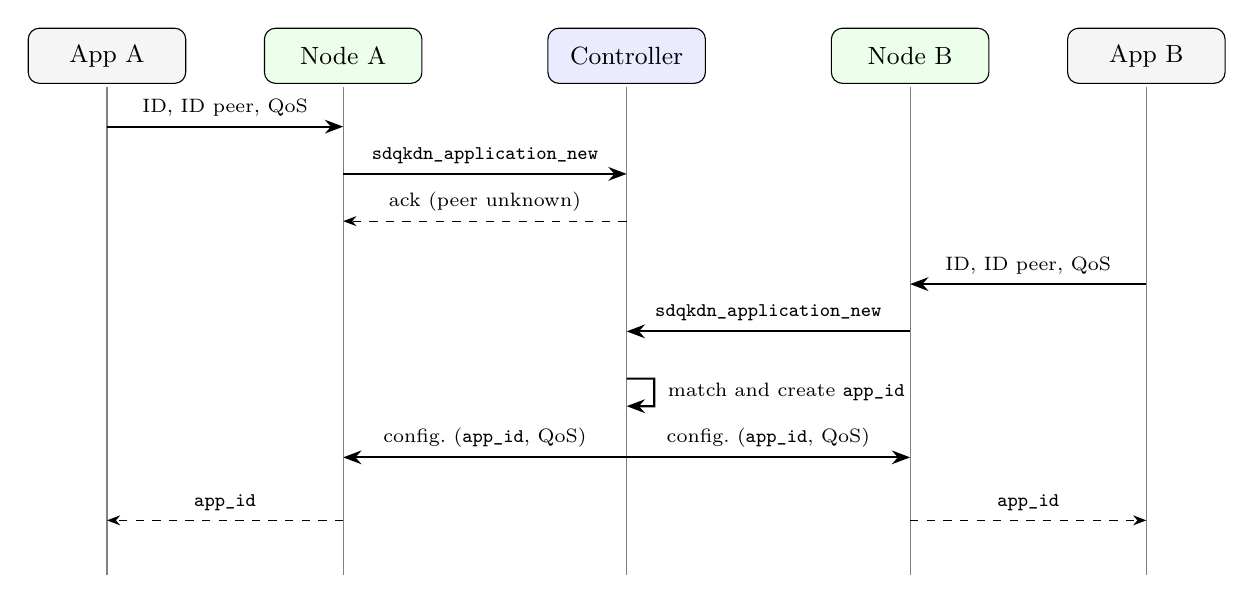
\begin{tikzpicture}[font=\scriptsize]
  \def\xA{0}\def\xB{3.0}\def\xC{6.6}\def\xD{10.2}\def\xE{13.2}
  \node[actor,minimum width=2cm] at (\xA,0) {App A};
  \node[actor,minimum width=2cm,fill=green!8] at (\xB,0) {Node A};
  \node[actor,minimum width=2cm,fill=blue!8] at (\xC,0) {Controller};
  \node[actor,minimum width=2cm,fill=green!8] at (\xD,0) {Node B};
  \node[actor,minimum width=2cm] at (\xE,0) {App B};
  \foreach \x in {\xA,\xB,\xC,\xD,\xE} \draw[gray] (\x,-0.4) -- (\x,-6.6);
  \draw[msg] (\xA,-0.9) -- node[above]{ID, ID peer, QoS} (\xB,-0.9);
  \draw[msg] (\xB,-1.5) -- node[above]{\texttt{sdqkdn\_application\_new}} (\xC,-1.5);
  \draw[ret] (\xC,-2.1) -- node[above]{ack (peer unknown)} (\xB,-2.1);
  \draw[msg] (\xE,-2.9) -- node[above]{ID, ID peer, QoS} (\xD,-2.9);
  \draw[msg] (\xD,-3.5) -- node[above]{\texttt{sdqkdn\_application\_new}} (\xC,-3.5);
  \draw[msg] (\xC,-4.1) -- ++(0.35,0) -- ++(0,-0.35) -- (\xC,-4.45);
  \node[right] at (\xC+0.4,-4.27) {match and create \texttt{app\_id}};
  \draw[msg] (\xC,-5.1) -- node[above]{config.\ (\texttt{app\_id}, QoS)} (\xB,-5.1);
  \draw[msg] (\xC,-5.1) -- node[above]{config.\ (\texttt{app\_id}, QoS)} (\xD,-5.1);
  \draw[ret] (\xB,-5.9) -- node[above]{\texttt{app\_id}} (\xA,-5.9);
  \draw[ret] (\xD,-5.9) -- node[above]{\texttt{app\_id}} (\xE,-5.9);
\end{tikzpicture}
\caption[Application registration in an SD-QKD network]{Application registration in an SD-QKD network. Applications
know only their own key manager; the controller matches the two requests
and creates the service identifier. Adapted from~\cite[Fig.~2]{qkd015}.}
\label{fig:seq015}
\end{figure}


\paragraph{Physical link creation.}
The controller receives a trigger, from a demand detected on the nodes or
from its own NBI. It looks for two free, compatible interfaces at the two
sites, asks the optical network controller (SD-ONC) for an optical path
(\emph{lightpath}) with the constraints of the quantum channel and, once
confirmed, configures the two interfaces on their nodes. If the two
controllers are merged into one, the operation is internal. This workflow
is the core of the QKD–optical network coexistence demanded by UC4.

\paragraph{Virtual link creation.}
If there are no compatible interfaces or no suitable lightpath, the
controller falls back to a virtual link. It computes a path over the
existing QKD network, for example on a weighted graph built from key
availability, generation rates and consumption; it configures each
intermediate node in relay mode, indicating previous and next hop; finally
it configures the endpoints with the bandwidth to provide. The
specification does not prescribe the algorithm. A natural choice,
consistent with~\eqref{eq:eskr015}, is to weight each link with the inverse
of its available key and discard links that cannot sustain the requested
bandwidth $r$:
\begin{equation}
  w_\ell = \frac{1}{\mathrm{ESKR}_\ell}, \qquad
  p^\star = \arg\min_{p\,:\,\min_{\ell\in p}\mathrm{ESKR}_\ell \ge r}
            \;\sum_{\ell\in p} w_\ell .
  \label{eq:path015}
\end{equation}
Equation~\eqref{eq:path015} is our example, not part of the standard. The
specification warns that, if poorly managed, virtual links can congest the
underlying physical links: this is precisely why a controller with a global
view of consumption and availability is needed.

% ---------------------------------------------------------------------
\subsubsection{Protocols and security}

GS~QKD~015 does not mandate a protocol, but points to the two most common
YANG-based ones: NETCONF~\cite{rfc6241}, typically between device and
controller, transactional and carried over SSH or TLS with XML encoding;
and RESTCONF~\cite{rfc8040}, typically on the controllers' NBI, based on
HTTP with CRUD operations and JSON or XML encoding.

On security (clause 6) the specification distinguishes two cases when a new
system is installed. If the system joins a secure site already in the
network, the channel to the controller can be protected with QKD keys
produced by existing links. If a new secure site is added, an initial
scheme (a trusted identity or a pre-shared secret, used only during
installation) is needed to introduce the new SDN agent to the controller;
after the first authentication, QKD keys take over. It is the same
key-growing principle seen at the beginning.

% ---------------------------------------------------------------------
\subsubsection{From a single domain to orchestration}

GS~QKD~015 solves the control of \emph{one} QKD domain by \emph{one}
controller. Three problems already hinted at by GS~QKD~002 are left out.
First, an operator may have several QKD domains, possibly from different
vendors, each with its own controller. Second, the applications that
consume key may live in another network, for example in the nodes of the
optical transport network, managed by a different controller. Third, the
operator wants to manage QKD with the same orchestration tools it uses for
the rest of the network. A higher layer is therefore needed, together with
a standard interface to reach it: this is the job of GS~QKD~018.

% =====================================================================
\section{ETSI GS QKD 018}
\label{sec:qkd018}
% =====================================================================

GS~QKD~018 (V1.1.1, April 2022)~\cite{qkd018} defines the
\emph{orchestration interface} between an SDN orchestrator and the SDN
controller of a QKD network. The controller acts as \emph{server}, the
orchestrator as \emph{client}; the information model is expressed in YANG
and is vendor-independent. In SDN terms it is the \emph{northbound
interface} of the QKD controller, i.e.\ the exact complement of
GS~QKD~015. The overall hierarchy becomes:
\begin{center}
\small
orchestrator $\xrightarrow{\text{QKD 018}}$ controller
$\xrightarrow{\text{QKD 015}}$ SDN agent / SD-QKD node
$\xrightarrow{\text{QKD 004/014}}$ SAE.
\end{center}

\begin{definition}[SDN orchestration]
\emph{SDN orchestration} is the continuous process by which available
resources are automatically coordinated, according to optimisation
criteria, to establish and release end-to-end services that span several
network domains, each governed by its own SDN
controller~\cite[§4.2]{qkd018}.
\end{definition}

\begin{definition}[Service link]
A \emph{service link} is a logical key association link between two QKD
nodes, realised by one or more physical QKD links (single-hop or
multi-hop). At the orchestration level it corresponds to the virtual link
of GS~QKD~015.
\end{definition}

% Figure: GS QKD 018 reference scenario (adapted from GS QKD 018, Fig. 1)
\begin{figure}[t]
\centering
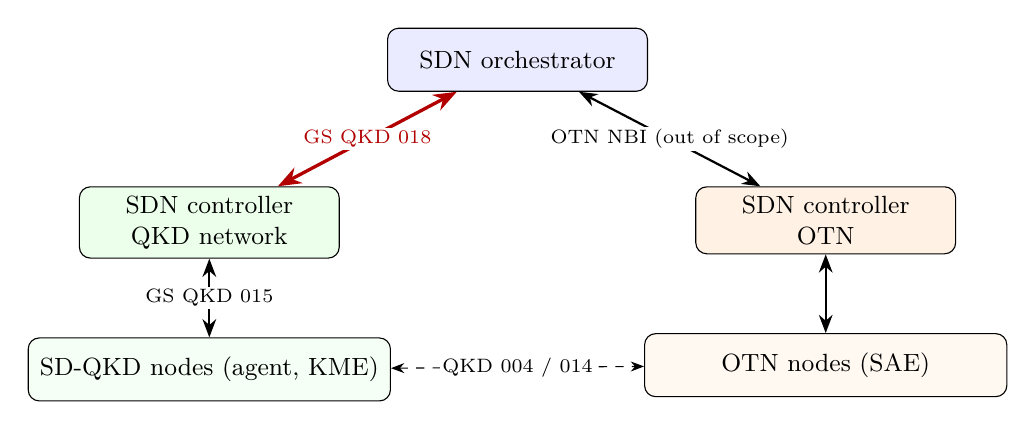
\begin{tikzpicture}
  \node[box,fill=blue!8,minimum width=3.3cm] (orch) {SDN orchestrator};
  \node[box,fill=green!8,minimum width=3.3cm,below left=12mm and 6mm of orch] (cq)
       {SDN controller\\QKD network};
  \node[box,fill=orange!10,minimum width=3.3cm,below right=12mm and 6mm of orch] (co)
       {SDN controller\\OTN};
  \node[box,fill=green!4,below=10mm of cq,minimum width=4.6cm] (nq)
       {SD-QKD nodes (agent, KME)};
  \node[box,fill=orange!5,below=10mm of co,minimum width=4.6cm] (no)
       {OTN nodes (SAE)};
  \draw[<->,very thick,red!70!black] (orch) -- node[lbl]{GS QKD 018} (cq);
  \draw[<->,thick] (orch) -- node[lbl]{OTN NBI (out of scope)} (co);
  \draw[<->,thick] (cq) -- node[lbl]{GS QKD 015} (nq);
  \draw[<->,thick] (co) -- (no);
  \draw[<->,dashed] (nq) -- node[lbl]{QKD 004 / 014} (no);
\end{tikzpicture}
\caption{GS~QKD~018 reference scenario (adapted
from~\cite[Fig.~1]{qkd018}). The standardised interface is in red; the
dashed line is key delivery from KMEs to SAEs, which happens inside the
same security perimeter.}
\label{fig:scenario}
\end{figure}


% ---------------------------------------------------------------------
\subsection{GS QKD 018 use cases}
\label{sec:usecase018}

The use case behind the standard (§4.1) takes up almost literally the
backbone problem of GS~QKD~002. An operator introducing QKD can either let
quantum and classical channels coexist in the same fibre or keep them
separate. Coexistence is hard for two reasons: the optical powers of
classical channels are many orders of magnitude higher and disturb the
quantum channel, and the reachable distances of the two kinds of channel
are very different. In a fibre-rich environment the operator may therefore
choose a QKD network separate from the optical transport network (OTN),
gaining performance, isolation and separation of responsibilities.
Following the SDN paradigm, the two networks are governed by different
controllers.

This creates a coordination problem: the SAEs that need to encrypt traffic
sit in OTN nodes, keys are generated in QKD nodes, and each controller knows
only its own network. The orchestrator solves three issues:

\begin{enumerate}
  \item \textbf{Address matching}: it pairs the address of the OTN node that
        must receive keys with that of the QKD node that supplies them; the
        two are inside the same security perimeter (Fig.~\ref{fig:scenario});
  \item \textbf{end-to-end provisioning}: it translates a customer request
        into the configuration of the individual domains, chooses the domains
        to traverse and coordinates the paths;
  \item \textbf{management}: it collects the topology, key-resource
        inventory and FCAPS information of each domain.
\end{enumerate}

Generalising, the same scheme makes it possible to orchestrate
\emph{several QKD domains from different vendors}, each behind its own
controller, as well as QKD and classical domains together. The standard
also points out a practical advantage: an operator that already has an
orchestrator for its optical networks can integrate the QKD network without
introducing separate management tools, which is exactly the integrated
management requirement of UC4.

The functions required of the orchestrator (§4.2) are:
\begin{itemize}
  \item translating customer service requests into domain configuration and
        SAE allocation;
  \item requesting establishment and release of services, including
        inter-domain connections;
  \item computing multi-domain paths, with inter-domain connections and
        endpoints;
  \item changing paths under operator constraints;
  \item discovering the nodes and links of each controller and keeping an
        abstract view of them;
  \item monitoring the key resources available on nodes and links;
  \item monitoring FCAPS management and receiving its notifications.
\end{itemize}

% ---------------------------------------------------------------------
\subsection{The information model}
\label{sec:infomodel}

Clause 5 translates these functions into five information blocks.

\paragraph{Topology discovery (§5.1).}
The controller exposes SD-QKD nodes, interfaces and physical links, and
later service links. The orchestrator does not need the full physical
composition, but an \emph{abstract} view of each domain and of the
connectivity between domains. Discovery can be \emph{proactive} (the
orchestrator queries the controller before every new path computation) or
\emph{reactive} (the controller notifies every change, e.g.\ a node added
or removed).

\paragraph{Network status and inventory (§5.2).}
For each node and physical link the controller exposes status, physical
performance and above all key resources: the generation rate and the rate
available after internal consumption. Service links add bandwidth,
available key and the restoration policy in case of failure.

\paragraph{End-to-end service status (§5.3).}
The orchestrator can query the active external applications, the local and
remote nodes and the service links that serve them, with their status and
key rate.

\paragraph{Provisioning with path computation (§5.4).}
The orchestrator asks the controller for paths that satisfy given
constraints; the controller returns a list of candidates, possibly several
times with different constraints, until the orchestrator picks one to
deploy. In case of failure the orchestrator can request the path to be
replaced.

\paragraph{Notifications (§5.5).}
The controller reports events, alarms and threshold crossings. Performance
thresholds (QBER, SKR, ESKR) are configurable by the orchestrator. Compared
with 015, notifications are added for node status (\texttt{sdqkdn\_new},
\texttt{\_operating}, \texttt{\_down}, \texttt{\_failure},
\texttt{\_out}), for deployed applications
(\texttt{sdqkdn\_application\_deployed}) and for service links
(\texttt{sdqkdn\_svc\_link\_down}, \texttt{\_perf\_update},
\texttt{\_overloaded}).

Equation~\eqref{eq:eskr015} extends naturally to the orchestration level.
Since in a multi-hop path $p$ every link relays the same key, a new service
with demand $r$ is sustainable only if the bottleneck can carry it:
\begin{equation}
  p \text{ admissible} \iff
  \min_{\ell\in p}\, \mathrm{ESKR}_\ell \;\ge\; r .
  \label{eq:admissible}
\end{equation}
This too is our own formalisation, consistent with the \texttt{skr},
\texttt{eskr} and \texttt{expected\_consumption} fields of the YANG models;
the standard does not prescribe any path-computation algorithm.

% =====================================================================
\subsection{The YANG modules}
\label{sec:yang018}
% =====================================================================

Annex~A (normative) turns the model into three YANG~1.1 modules, published
on ETSI Forge~\cite{qkd018yang}. With the constructs seen in
§\ref{sec:yang-anatomia} their structure is quick to read. The modules
import \texttt{etsi-qkd-sdn-node} and \texttt{etsi-qkd-node-types} from
GS~QKD~015 to reuse their types (identifiers, link types, application QoS):
018 does not reinvent the node, it provides an abstract view of it. The
three modules form a chain: \emph{topology} (the skeleton) $\to$
\emph{inventory} (what is there and in which state) $\to$
\emph{connectivity} (what is done with it).

\paragraph{\texttt{etsi-qkd-sdn-topology} (prefix \texttt{qkdnw-tplg}).}
It describes only the structure, i.e.\ who is connected to whom:
\begin{lstlisting}
qkd_network
 +-- sdqkd_nodes
 |    +-- qkdn* [qkdn_id]                          SD-QKD nodes
 |         +-- qkd_interfaces/qkdi* [qkdi_id]      QKD modules
 +-- qkd_links
      +-- qkd_phys_links/phys_link* [phys_link_id]  physical links
      |    +-- link_type
      |    +-- phys_link_local_qkdn   (qkdn_id_ref, qkdi_id_ref)
      |    +-- phys_link_remote_qkdn  (qkdn_id_ref, qkdi_id_ref)
      +-- qkd_svc_links/svc_link* [svc_link_id]     service links
           +-- ... local/remote endpoints as above
\end{lstlisting}
Compared with 015 the point of view changes: there is no longer a tree per
node, but a single tree for the whole network of the domain. Abstractly it
is a graph $G=(V,E)$ with $V$ the set of \texttt{qkdn} nodes and
$E = E_{\text{phys}}\cup E_{\text{svc}}$, where \texttt{phys\_link}s
represent physical adjacencies and \texttt{svc\_link}s logical key
relations, possibly multi-hop. Endpoints are \texttt{leafref}s, i.e.\
validated references to existing nodes and interfaces. Given the graph
$G_i$ of each domain $i$, the orchestrator composes a multi-domain view
\begin{equation}
  G = \Big(\bigcup_i V_i,\; \bigcup_i E_i \,\cup\, E_{\text{inter}}\Big),
\end{equation}
where $E_{\text{inter}}$ are the adjacencies between domains, typically
realised by shared border nodes.

\paragraph{\texttt{etsi-qkd-sdn-inventory} (prefix \texttt{qkdnw-invt}).}
It does not create a new tree but \texttt{augment}s the topology tree,
adding leaves to elements already defined (Table~\ref{tab:inventory}). It
is a textbook use of \texttt{augment}: those interested only in the
structure implement the topology, those who also want the state add the
inventory without duplicating anything.

\begin{table}[h]
\centering\small
\caption{Elements added by the inventory module to the topology tree.}
\label{tab:inventory}
\begin{tabularx}{\textwidth}{@{}l L@{}}
\toprule
\textbf{Element} & \textbf{Added leaves} \\
\midrule
\texttt{qkdn} & version, capabilities, location, KME IP address and port
(where SAEs fetch keys via QKD~014), status \\
\texttt{qkdi} & supported role, model, type, attachment point, status \\
\texttt{phys\_link} & \texttt{enable} (configurable), \texttt{wavelength},
\texttt{performance} (\texttt{skr}, \texttt{eskr},
\texttt{expected\_consumption}, QBER, SNR), status \\
\texttt{svc\_link} & \texttt{bandwidth}, \texttt{performance},
\texttt{path\_restoration} (\texttt{AUTOMATIC}/\texttt{MANUAL},
\texttt{hold\_off\_time} in ms), status \\
\bottomrule
\end{tabularx}
\end{table}

The module also defines the notifications that implement the reactive part
of §5.5: \texttt{sdqkdn\_new}, \texttt{sdqkdn\_interface\_new},
\texttt{sdqkdn\_phys\_link\_new}, \texttt{sdqkdn\_svc\_link\_new}, the
\texttt{\_perf\_update} and \texttt{\_overloaded} variants and the generic
\texttt{alarm} and \texttt{event}. The \texttt{eskr} field of the links is
what tells the orchestrator whether a path can carry a new service,
according to~\eqref{eq:admissible}.

\paragraph{\texttt{etsi-qkd-sdn-connectivity} (prefix \texttt{qkdnw-conn}).}
This is the operational module: it manages applications and the paths that
serve them.
\begin{lstlisting}
connectivity_service/qkd_service/qkd_app* [app_id]
 +-- (application data from QKD 015: status, type, QoS, statistics)
 +-- app_mapped_svc_link
      +-- svc_link_and_qkdn_ids   service link and endpoints
      +-- path_constraints        include_nodes / exclude_nodes
      +-- candidate_paths         num_of_candidate_paths + list of paths
      +-- deploy_path             chosen path_id
\end{lstlisting}
Here the \texttt{rpc}s appear, mirroring the provisioning workflow step by
step:
\begin{description}[font=\normalfont\ttfamily\footnotesize,style=nextline,leftmargin=1.2em]
  \item[app-registration] registers the application in the domain;
  \item[create-service-link-id-for-app] creates the service link between
        local and remote node;
  \item[create-candidate-paths-per-service-link-for-app] the controller
        computes candidate paths honouring QoS and the
        \texttt{include\_nodes}/\texttt{exclude\_nodes} constraints;
  \item[update-candidate-paths-per-service-link-for-app] recomputation with
        different constraints;
  \item[deploy-a-candidate-path-per-service-link-for-app] the orchestrator
        picks a \texttt{path\_id} and the controller activates it;
  \item[delete-deployed-path-per-service-link-for-app] releases the path.
\end{description}
The module's notifications are \texttt{sdqkdn\_application\_new},
\texttt{sdqkdn\_application\_deployed},
\texttt{sdqkdn\_application\_qos\_update} and
\texttt{sdqkdn\_application\_disconnected}.

The conceptual point is the \textbf{division of roles}: the controller
knows its own domain and \emph{proposes} paths, the orchestrator has the
overall view and \emph{decides}. Table~\ref{tab:moduli} sums up.

\begin{table}[h]
\centering\small
\caption{The three YANG modules of GS~QKD~018.}
\label{tab:moduli}
\begin{tabularx}{\textwidth}{@{}l L l L@{}}
\toprule
\textbf{Module} & \textbf{Question} & \textbf{Clause} & \textbf{Data} \\
\midrule
topology & What does the network look like? & §5.1 & structure (graph) \\
inventory & How many resources, in which state? & §5.2, §5.5 &
status, performance, configuration, notifications \\
connectivity & How do I serve an application end to end? & §5.3, §5.4, §6.2 &
applications, path computation and deployment RPCs \\
\bottomrule
\end{tabularx}
\end{table}

% =====================================================================
\subsection{Multi-domain provisioning workflow}
\label{sec:workflow}
% =====================================================================

Clause 6 ties the information to the service life cycle. When the QKD
network is introduced, the orchestrator acquires its topology (§5.1);
during operation it receives status and inventory, on demand or
periodically (§5.2); after a service is activated it monitors its status
(§5.3); at any time it receives notifications (§5.5).

§6.2 describes the complete case (Fig.~\ref{fig:seq018}): an orchestrator
coordinates the QKD controller and the OTN controller, which do not talk to
each other directly.

% Figure: end-to-end QKD + OTN provisioning (adapted from GS QKD 018, Fig. 2)
\begin{figure}[t]
\centering
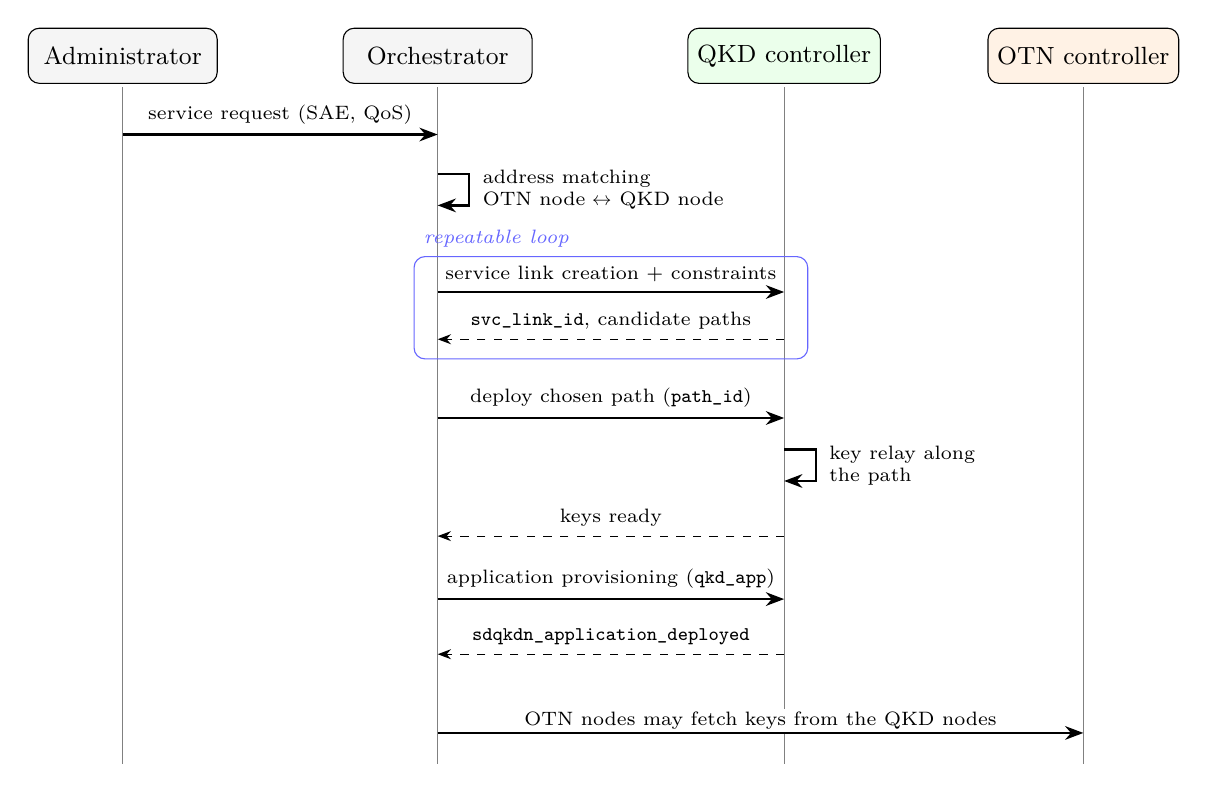
\begin{tikzpicture}[font=\scriptsize]
  \def\xA{0}\def\xB{4.0}\def\xC{8.4}\def\xD{12.2}
  \node[actor] at (\xA,0) {Administrator};
  \node[actor] at (\xB,0) {Orchestrator};
  \node[actor,fill=green!8] at (\xC,0) {QKD controller};
  \node[actor,fill=orange!10] at (\xD,0) {OTN controller};
  \foreach \x in {\xA,\xB,\xC,\xD} \draw[gray] (\x,-0.4) -- (\x,-9.0);
  \draw[msg] (\xA,-1.0) -- node[above]{service request (SAE, QoS)} (\xB,-1.0);
  \draw[msg] (\xB,-1.5) -- ++(0.4,0) -- ++(0,-0.4) -- (\xB,-1.9);
  \node[right,align=left] at (\xB+0.45,-1.7) {address matching\\OTN node $\leftrightarrow$ QKD node};
  \draw[blue!60,rounded corners] (\xB-0.3,-2.55) rectangle (\xC+0.3,-3.85);
  \node[blue!60,anchor=south west,font=\scriptsize\itshape] at (\xB-0.3,-2.55) {repeatable loop};
  \draw[msg] (\xB,-3.0) -- node[above]{service link creation + constraints} (\xC,-3.0);
  \draw[ret] (\xC,-3.6) -- node[above]{\texttt{svc\_link\_id}, candidate paths} (\xB,-3.6);
  \draw[msg] (\xB,-4.6) -- node[above]{deploy chosen path (\texttt{path\_id})} (\xC,-4.6);
  \draw[msg] (\xC,-5.0) -- ++(0.4,0) -- ++(0,-0.4) -- (\xC,-5.4);
  \node[right,align=left] at (\xC+0.45,-5.2) {key relay along\\the path};
  \draw[ret] (\xC,-6.1) -- node[above]{keys ready} (\xB,-6.1);
  \draw[msg] (\xB,-6.9) -- node[above]{application provisioning (\texttt{qkd\_app})} (\xC,-6.9);
  \draw[ret] (\xC,-7.6) -- node[above]{\texttt{sdqkdn\_application\_deployed}} (\xB,-7.6);
  \draw[msg] (\xB,-8.6) -- node[above,fill=white,inner sep=1pt]{OTN nodes may fetch keys from the QKD nodes} (\xD,-8.6);
\end{tikzpicture}
\caption[End-to-end provisioning of a QKD service across a QKD network and an OTN]{End-to-end provisioning of a QKD service across a QKD network and
an OTN (simplified from~\cite[Fig.~2]{qkd018}). The interaction with the
OTN controller is out of the scope of the specification.}
\label{fig:seq018}
\end{figure}


The steps are:
\begin{enumerate}
  \item the administrator requests a service from the orchestrator,
        specifying the SAEs in the OTN nodes and their QoS;
  \item the orchestrator identifies the controllers involved and performs
        address matching; it already knows the addresses of the QKD nodes
        thanks to topology and inventory;
  \item it asks the QKD controller to create a service link and compute
        paths, with the desired constraints;
  \item the controller assigns an \texttt{svc\_link\_id} and returns the
        candidate paths, each with a priority; this step may be repeated
        with different constraints;
  \item the orchestrator picks a path and requests its deployment; the
        nodes generate and relay keys along the path until both ends are
        ready;
  \item once confirmed, the orchestrator requests provisioning of the
        application on the service link and tells the OTN controller that
        the OTN nodes may start fetching keys from the designated QKD
        nodes.
\end{enumerate}
Note the parallel with the virtual-link workflow of 015: there the
controller computed and configured the path on its own, here it
\emph{proposes} it and waits for the orchestrator's choice. With several
QKD domains the orchestrator repeats steps 3–5 for each domain along the
chosen inter-domain path, joining the segments through border nodes: this
is what Sim et al.\ do (§\ref{sec:sim}).

% =====================================================================
\subsection{Protocols and security}
\label{sec:protocolli}
% =====================================================================

\paragraph{Transport (§8).}
Like 015, the standard separates the data model (YANG~1.1) from the
transport protocol, which can be NETCONF~\cite{rfc6241} or
RESTCONF~\cite{rfc8040}. With RESTCONF every resource is a URI, reads use
\texttt{GET} and configuration uses \texttt{POST}, \texttt{PUT},
\texttt{PATCH} and \texttt{DELETE}, with XML or JSON encoding;
notifications are received by subscribing to the corresponding streams.
The standard notes that the stateless REST paradigm suits this kind of API.
As an example, reading the topology and invoking an RPC would look like:
\begin{lstlisting}
GET  /restconf/data/etsi-qkd-sdn-topology:qkd_network
POST /restconf/operations/etsi-qkd-sdn-connectivity:create-service-link-id-for-app
\end{lstlisting}

\paragraph{Security (§7).}
The controller has a central view of the network and passes a subset of it
to the orchestrator; protection measures for the interface (authentication,
channel encryption, e.g.\ TLS under RESTCONF) are left to implementations.
The fundamental principle, inherited from GS~QKD~015, is that
\textbf{QKD-derived keys never pass through either the controller or the
orchestrator}: the YANG modules contain only key rates and the KME address.
A compromised orchestrator can therefore cause service disruption (wrong
paths, exhausted resources, denial of service) but cannot read keys. The
standard recommends careful design, installation and personalisation
procedures to mitigate malicious requests and attacks on control channels.

% =====================================================================
\section{The analogy with ACTN (RFC 8453)}
\label{sec:actn}
% =====================================================================

GS~QKD~018 does not invent a new model: it applies to QKD a pattern that is
already standard in transport networks, the IETF ACTN framework
(\emph{Abstraction and Control of TE Networks})~\cite{rfc8453}. ACTN has
three levels: the \emph{Customer Network Controller} (CNC), the
\emph{Multi-Domain Service Coordinator} (MDSC) and the per-domain
\emph{Provisioning Network Controllers} (PNC), connected by the CMI
(CNC–MDSC) and MPI (MDSC–PNC) interfaces. The mapping to GS~QKD~018 is
direct (Table~\ref{tab:actn}).

\begin{table}[h]
\centering\small
\caption{Mapping between ACTN and the ETSI QKD stack.}
\label{tab:actn}
\begin{tabularx}{\textwidth}{@{}l l L@{}}
\toprule
\textbf{ACTN} & \textbf{ETSI QKD} & \textbf{Remark} \\
\midrule
CNC & administrator / customer portal & originates the service request \\
MDSC & SDN orchestrator & multi-domain view, path decision \\
PNC & SDN controller of the QKD domain & computes candidates, activates paths \\
MPI & GS~QKD~018 interface & abstract topology, provisioning, notifications \\
SBI & GS~QKD~015 interface & control of individual nodes \\
abstract TE topology & \texttt{etsi-qkd-sdn-topology} & vendor-neutral view \\
TE bandwidth & SKR / ESKR & the resource to allocate is key \\
\bottomrule
\end{tabularx}
\end{table}

The essential difference lies in the resource. In ACTN the bandwidth of a
link is fixed by the channel capacity; in QKD the SKR fluctuates with
physical conditions and key accumulates in finite buffers from which it is
consumed. This is why in 018 notifications such as \texttt{\_perf\_update}
and \texttt{\_overloaded} and the \texttt{path\_restoration} policy play a
more central role than in classical transport networks.

% =====================================================================
\section{Real deployments}
\label{sec:casi}
% =====================================================================

\subsection{SK Telecom: multi-vendor orchestration on KOREN}
\label{sec:sim}

Sim et al.~\cite{sim2023} describe the first documented commercial
deployment of a GS~QKD~018-compliant orchestrator, on the testbed of the
Korean research network KOREN (2020–2022). Two QKD operators run two
networks with devices and KMSs from different vendors, each with its own
controller (QKDNC); an orchestrator (QKDNO) coordinates them. Links use
decoy-state BB84 over spans between $39$ and $100$~km. The two networks meet
at \emph{border nodes} (e.g.\ Pangyo and Daejeon) that contain no QKD
modules but two interconnected KMSs, one per operator.

When two SAEs belong to different networks, the orchestrator computes the
end-to-end path with a \emph{path computation engine}, choosing \emph{in
advance} the border node to traverse; each controller then creates its own
service-link segment. To bind the segments the authors extend the model:
they introduce a \emph{multi-segment} application type (\texttt{MS}), with
an identifier \texttt{ms\_app\_id} shared across domains and
\texttt{server\_ms\_info} and \texttt{client\_ms\_info} describing the
external KMSs, plus an \texttt{app-registration-ms} RPC. Key transfer at
the border node uses the KMS–KMS interface of GS~QKD~020~\cite{qkd020}.
The case shows both the soundness of the 018 scheme and one of its limits:
the application types inherited from 015 (\texttt{CLIENT} and
\texttt{INTERNAL}) are not enough for multi-domain, and extensions are
needed. It is also a good illustration of the usefulness of the YANG
\texttt{identity} construct discussed in §\ref{sec:yang-anatomia}: a new
type can be added without rewriting the original model.

\subsection{Politecnico di Milano: hierarchical control with ONOS}

Vicario's thesis~\cite{vicario2025} builds an end-to-end prototype of
hierarchical control for metropolitan networks: the domain controllers are
based on ONOS and manage the nodes through the GS~QKD~015 model, while the
upward interface is GS~QKD~018, exposed via RESTCONF to a Python
orchestrator that aggregates the topology of several domains. It is a
useful implementation because it shows the whole 015~$\to$~018 stack in
open software, with the same YANG modules described in §\ref{sec:yang018}.

\subsection{MadQCI: the Madrid network}

MadQCI~\cite{madqci2024} is a real QKD network in Madrid with dozens of
modules from different vendors over more than $130$~km, integrated with the
production optical network. Control relies on an SD-QKD stack based on
GS~QKD~015, which is confirmed as the most widely adopted standard.
GS~QKD~018 is mentioned as a tool for inter-domain orchestration and
optical–quantum coordination, but the authors describe it as work still in
progress. This is an honest picture of the state of the art: domain control
is mature, orchestration much less so.

% =====================================================================
\section{Limits and outlook}
\label{sec:limiti}
% =====================================================================

\begin{itemize}
  \item \textbf{Adoption.} 015 is used in real networks, 018 almost only in
        testbeds and prototypes~\cite{madqci2024}.
  \item \textbf{Incomplete multi-domain support.} The normative scenario is
        QKD$+$OTN; the QKD$+$QKD case requires extensions like those of Sim
        et al.\ and coordination with GS~QKD~020 for key hand-over between
        KMSs.
  \item \textbf{Metrics.} ESKR is an instantaneous indicator and accounts
        neither for key already accumulated in buffers nor for its
        dynamics. Laschet et al.~\cite{laschet2026} propose richer
        indicators for path selection.
  \item \textbf{Topology confidentiality.} Exposing the internal topology
        to the orchestrator is acceptable within one operator, less so
        between different operators; inter-domain routing schemes that
        preserve confidentiality are needed~\cite{laschet2026,interconnect2026}.
  \item \textbf{Interface security.} The standard does not specify how the
        orchestrator–controller channel is protected, leaving it to
        implementations.
  \item \textbf{Algorithms.} Path computation is not standardised: this
        helps innovation~\cite{routing2024,mendez2026} but makes behaviour
        less predictable in multi-vendor scenarios.
\end{itemize}

% =====================================================================
\section{Conclusions}
\label{sec:conclusioni}
% =====================================================================

Read in sequence, ETSI's work on QKD control follows a clear logic.
GS~QKD~002 showed that useful QKD is a network, with key management,
differentiated service requirements and integration into the operator's
optical network. GS~QKD~015 answered with the SD-QKD node abstraction:
modules as interfaces, a single key manager, physical and virtual links,
applications with QoS, and a controller that registers, plans and
configures, all described in YANG. GS~QKD~018 added the orchestration
layer: each domain becomes an abstract graph, key resources are monitored
through the inventory and provisioning follows a scheme in which the
controller proposes and the orchestrator decides. The design mirrors ACTN,
reuses YANG, NETCONF and RESTCONF and keeps the essential security
principle: keys never leave the nodes. The KOREN, Politecnico di Milano and
MadQCI experiences show that the scheme works but that QKD orchestration is
still young. The next step is to truly extend it to multi-operator
settings, with better metrics and confidentiality guarantees between
domains.


\printbibliography[heading=bibintoc,title={References}]

\end{document}
